\title{DLX }
\documentclass[12pt]{article}
\usepackage[T1]{fontenc}
\usepackage{graphicx}
\usepackage{lscape}

\usepackage{listings}
\usepackage{epstopdf}
\usepackage[dvipsnames]{xcolor}
\usepackage{colortbl}
\usepackage[export]{adjustbox}
\usepackage[section]{placeins}

\usepackage[style=numeric-comp]{biblatex}
\bibliography{document.bib}

\setlength{\parindent}{0pt}
\lstset{
	breaklines=true,
	numbersep=5pt,
	xleftmargin=.25in} 

\begin{document}
\maketitle
\tableofcontents

\section{Introduction}
The goal of this project is to implement an RTL completely functional DLX processor in VHDL, simulate it and then proceed with the design flow with synthesis and layout phases.

DLX processor architecture was designed by John L. Hennessy and David A. Patterson\cite{Patterson:1990:CAQ:77493} and very well described and documented all over the internet.

This project is developed for the course Microelectronic Systems taught by Prof. Mariagrazia Graziano in Politecnico di Torino\cite{MGLECTURENOTES}.



\paragraph{Outline}
The remainder of this article is organized as follows:
 
I will first give a brief overview of the DLX architecture and my personal implementation in Section~\ref{Overview}.
In Section~\ref{Design} will go into details regarding particular aspects of the datapath and control unit.
Section~\ref{Synthesis} and~\ref{Layout} are about the environment and results of design and layout phases.
Finally, Section~\ref{Conclusions} gives the conclusions and possible future work.

\section{Implmentation Overview}\label{Overview}
DLX is a classic 5-stage pipelined processor, with fixed length instructions and in-order execution.
Most information regarding the ISA, structure and description of operations can be found in \cite{ISA}.
\paragraph{Instructions}
In this version, all I-TYPE and R-TYPE operations have been implemented with the exception of: LHI, RFE, TRAP, ITLB, LB, LH, LBU, LHU, LF, LD, SB, SH, SF, SD and all MOV operations.

The only F-TYPE instructions implemented are MULT and MULTU, but they operate on integer register instead of floating point ones.

During normal conditions, all operations take exactly 5 cycles to execute, with the exception of multiplications, which require a fixed amount of 14 cycles (10 cycles are spent in the execute stage) and they're not pipelineable.

\paragraph{Jump and branch}
Jump and Branch instructions target address is aggressively evaluated in the decode stage in order to have less cc penalty.
In addition to this, a 2-bit predictor scheme has been implemented. This will be discussed more in the next section.

\paragraph{Control logic}
The execution is regulated by an hardwired CU, in charge of producing control words for each stage of the pipeline, as well as stall signals to stop the execution when needed.
All possible hazards have been solved through a forwarding logic, when this is not enough, a stall signal is sent from the control unit to the registers that need to be stalled.

\paragraph{Memories}
Two separated memories for instruction and data have been included in the design, but they are actually not part of it because they are always external peripherals.
\begin{itemize}
\item Instruction memory is asynchronous, with 1 read port. Write is not possible.
\item Data memory is synchronous, with 1 read port and 1 write port. Concurrent write and read is not possible.
\end{itemize}

\paragraph{Register file}
Register file has 2 read port and one write port. Concurrent write and read on the same register produces a redirection of the input data to the output.

\section{Design Architecture}\label{Design}
As previously mentioned, the processor is described in VHDL. Most blocks are written in a structural approach up to very basic logic elements such as multiplexers, half adders, etc \ldots

An overview of the processor architecture is shown in FIGUREXXX at the end of this document.

In the next sections we are going to see in details each single component.

\subsection{Fetch Block}
\begin{figure}[h!]
	\includegraphics[width=\textwidth, center]{images/FETCH_BLOCK.eps}
	\caption{Fetch Block Schematic}
	\label{FETCHBLOCK}
\end{figure}
Fetch block is in charge of correctly fetch the instruction to be executed from the memory. This block is tightly coupled with branch predictor. As can be seen in the picture, the actual decision of the next PC to drive comes from the BTB in case of normal operations.

MUXTARGET computes the correct target pc, which is sent to the branch predictor to evaluate the misprediction signal that controls MUXPRED.
When misprediction signal is triggered, the current operation in the PC is fetched but not sent to decode stage, and it is replaced by the correct one on the successive clock cycle.

\subsection{Branch Predictor}
\begin{figure}[h!]
	\includegraphics[width=\textwidth, center]{images/BTB.eps}
	\caption{BTB}
	\label{Branch Predictor Block Schematic}
\end{figure}
As previously stated, a branch predictor scheme has been applied, in particular it is a 2bit saturating counter BHT, also widely known in literature as (0,2). In addition, we have also implemented a BTB in charge of storing the PC of the next instruction in case the branch is taken.

The design applied is very generic, so the number of entries is easily configurable.

In normal situations the lowest part of the PC, called TAG, is used to index the BTH, if the instruction is recognized as a taken branch, then the PC found inside the BTB is sent to the fetch block. On the successive clock cycle, when the decode block actually computed the correct behavior of the branch, the value of the BTH is updated and, if the prediction was not correct, mispredict signal is triggered.
Also, due to the fact that mispredict signal actually cause the current operation in the fetch stage to be re-evaluated, the branch predictor automatically disables itself on the following clock cycle to avoid possible deadlock conditions.

Some information regarding the operations performed on the last clock cycle need to be stored, to do so, 4 have been added, they store: prediction, prediction target, TAG and mispredict signals.

\subsection{Decode Block}
\begin{figure}[h!]
	\includegraphics[width=\textwidth, center]{images/DECODE_BLOCK.eps}
	\caption{Decode Block Schematic}
	\label{DECODEBLOCK}
\end{figure}
Decode block is in charge of 4 main functions:
\begin{itemize}
	\item Split from IR register number values rA, rB and rC used in the next stage and for forwarding.
	\item Extend the immediate to 16/26 bits, either signed or unsigned, according to the current decoded instruction.
	\item Compute the addition between NPCF and the offset given by the extended immediate value
	\item Evaluate branch output through the zero comparator, the negation of this signal is also sent to other components in the system.
\end{itemize}
In case of Jump operations with link ( JAL and JALR ) the immediate value is replaced by the return address by MUXLINK.

\subsection{Execute Block}
\begin{figure}[ht!]
	\includegraphics[width=\textwidth, center]{images/DLX_ALU.eps}
	\caption{ALU and Multiplier Block Schematic}
	\label{ALU}
\end{figure}
Execute block is third stage of the pipeline. Most of the computation done here is due to the ALU which will be explored in detail in the next section.

For the moment let's also forget about forwarding multiplexers, as they are going to be described later.

ALU is fed with two operands: one is always A, while the other could come wither from B or IMM, depending on the type of operation. A multiplexer is then added to achieve this functionality.
The multiplexed value is also sent directly to output, it is going to feed the Data memory input in the next stage.

Another multiplexer (DESTMUX) is also used to select in which destination register the current operation is going to write. Again, there is difference between I-TYPE and R-TYPE operations, and also a special input is due to JAL and JALR instructions that have R31 as a forced destination register.

 
\subsection{ALU and Multiplier}
The ALU is responsible for all data manipulation and it's the heart of our processor.

It takes as input two 32 bit operands and a special sequence of control bits generated in the decode stage. The ALU is not directly fed with the ALU opcode for performance reasons ( This was a bottleneck in an early version of the ALU, and there is no need to generate the control bit in the execute stage ).
The output consist in the 32 bit result and a signal that is at logic '1' during multi cycle operations.

Carry out has been suppressed because in this architecture is never used (unless for comparison operations).

The ALU is composed of the following units:

\begin{itemize}
	\item A single shared adder
	\item Multiplication logic
	\item Logic Unit
	\item Comparator
	\item Shifter
\end{itemize}

The results coming from these units is then multiplexed to the final output.
We are going to see in details each of them in the next sections.

\subsubsection{Shared Adder}
The adder/subtractor is a 32-bit Pentium 4 adder.

It is composed of two main blocks: 
\paragraph{Sparse tree}The Sparse tree is in charge of computing all carries in a parallel fashion. In our case it is a radix-2 carry-merge tree and generates every fourth carry. 

\paragraph{Sum generator}The sum generator block is then based on carry select adders, which compute both results in case the carry is 0 and in case the carry is 1. These two addition are independent from the actual carry, so they can be performed in parallel. When the carry reaches the sum generator it controls a multiplexer used to select one of the two possible outputs.
As a consequence, the delay due to carry propagation is strongly minimized.
\newline
\newline
In order to perform subtractions, a little modification has been applied. From basic computer arithmetic we know that subtracting is the same as doing an addition with the second operand being 2's complemented.

2's complement involves doing a not of the entire number and adding 1.
Flipping of the bits is performed with a xor circuit placed at the input of the second operand, while the 1 addition is done trough the carry input. ( carry input would never been used in this specific architecture ). 



\subsubsection{Multiplier Logic}
As briefly introduced, Multiplication is performed by the shared P4 adder in an iterative way.
The entire procedure is based on the Booth's multiplier. Instead of producing all the sums in parallel, we compute one each clock cycle.
To avoid using 64 bits registers to store a 32x32 multiplication, only the lowest 16-bits of the two operands are considered.

The flow is as follows:
At the first clock cycle all the Booth's encoding is done and sent in a PISO register, also value of A is saved into a register able to left shift it's content of 2 every clock cycle (multiplying by 4). Accumulator register is cleaned and set to zero.

Then at each clock cycle the adder takes as input the correctly shifted input value and the result of the previous addition stored in the accumulator register. When a subtraction needs to be performed, the carry input of the adder is set to '1'.
To have both signed and unsigned multiplication, a correction stage needs to be performed at the end, as can be seen in the picture, the last encoder takes this into account.

Please also note that a little modification to the booth encoding pattern has been made in order to have a direct mapping between bits and function. Have a look at Table \ref{BOOTHENC}.
\begin{table}
\begin{center}
	\begin{tabular}{ | c | c | c |}
		\hline
		\rowcolor{LimeGreen} Input & Encoding & Action \\ \hline
		000 & 000 & +0 \\ \hline
		001 & 100 & +A \\ \hline
		010 & 100 & +A \\ \hline
		011 & 101 & +2A \\ \hline
		100 & 111 & -2A \\ \hline
		101 & 110 & -A \\ \hline
		110 & 110 & -A \\ \hline
		111 & 000 & 0 \\ \hline
		
	\end{tabular}
	\caption{Modified Booth Encoding}
	\label{BOOTHENC}
\end{center}
\end{table}

Bit explanation (MSB to LSB):
\begin{itemize}
	\item First bit tells us whether or not we actually need to use the adder. This bit is directly sent to the enable of the accumulator, if it is '0', there is no need to sample the new value received from the adder.
	\item Second bit tells to the adder if it need to compute an addition or a subtraction. This bit is sent both to the sign and the carry in of the adder. '0' stands for addition, while '1' is for subtraction
	\item Finally the last bit decides the input of the adder. '0' is for the clean value straight of A register, while '1' is used when we need the value left-shifted by 1 position. This bit controls INPUTMUX.
\end{itemize}

This design is able to reduce critical paths flowing to a standard parallel multiplier and save area as well at the cost of a multi cycle operation. 

We put a lot of effort into optimization for this part of the design. The first image shows the initial design, while the latter the final version. Please also consider that we decided to move from 9 to 10 cycles to reduce the critical path.
A possible future improvement could be to pipeline the Booth Encoder block too to save area.

We have thought a lot of possible ideas to improve this design from a power-reduction point of view. Unfortunately, most of the possible improvements require latches, and these kind of components are not simple to handle, both for simulation and synthesis aspect.

This is due to the asynchronous behavior of latches and the possible race conditions that might happen in a circuit with latches and flip-flops. We tried something, unfortunately all our efforts achieved nothing and we discarded the idea.

\subsubsection{Logic Unit}
The DLX architecture supports only 3 type of logical operations: AND, OR, XOR. 
\begin{figure}[h]
	\includegraphics[center]{images/LOGIC_UNIT.eps}
	\caption{Logic Unit Schematic}
	\label{LU}
\end{figure}
Due to this simple behavior, we decided to avoid using particular logic unit schemes: the three operations are executed in parallel and then a multiplexer selects the correct one. 

As can be see in the picture, the schematic is pretty straightforward.


\subsubsection{Comparator}
The ISA requires to implement several comparison operation: $(<, >, \leq, \geq, =, \neq)$.
Dealing with both signed and unsigned numbers is not easy in a comparator, because the two operations use different inputs.

For a comparison the required signals are:
\begin{itemize}
	\item difference between the two numbers, provided by the shared ALU (SUM)
	\item carry out of the operation (C)
	\item overflow bit (V)
	\item sign
\end{itemize}
Overflow bit is computed outside of the comparator as (IN2(31) xnor SUM(31)) and (IN1 xor IN2).
Which basically mean that an overflow is triggered when subtrahend and result have the same sign when minuend and subtrahend have different sign.

Zero bit (Z) is computed through nor reduction of SUM, while the sign of SUM (N) is simply the most significant bit.
\begin{table}
\begin{center}
	\begin{tabular}{ | l | l | l |}
		\hline
		\rowcolor{LimeGreen} OP & Description & Flags tested \\ \hline
		SEQ & Equal & Z \\ \hline
		SNE & Not equal &  not Z \\ \hline
		SGT & Signed greater & N xnor V \\ \hline
		SGE & Signed greater or equal & (N  xnor  V) or Z \\ \hline
		SLT & Signed less & (N xor V) and (not Z)\\ \hline
		SLE & Signed less or equal & N xor V \\ \hline
		SGTU & Unsigned greater & C and (not Z) \\ \hline
		SGEU & Unsigned greater or equal & C \\ \hline
		SLTU & Unsigned less & not C \\ \hline
		SLEU & Unsigned less or equal & (not C) or Z  \\ \hline
	\end{tabular}
		\caption{Comparison Signals}
		\label{COMPA}
\end{center}
\end{table}

There might be some redundancies in the design, we left possible optimizations to the synthesizer.

\subsubsection{Shifter}
\begin{figure}[t]
	\includegraphics[width=\textwidth, center]{images/SHIFTER.eps}
	\caption{Shifter Block Schematic}
	\label{SHIFTER}
\end{figure}
The DLX-basic shift operations are: SLL, SRL, SRLI, SRA and SRAI, actually our hardware would be able to implement also the missing ones.
Our implementation is based on the T2 coarse-grain shifter and is organized on three different blocks:
\begin{itemize}
	\item Level 1: this block produces three masks according to the selection signal (00, 01 or 10).
	shifted by 0 (mask0), 8 (mask8) and 16 bits (mask16) each. Moreover, operand IN1 is extended
	to 39 bits.
	\paragraph{00 :} the operand is shifted left replacing vacant positions with 0s and extended appending
	7 0s to the right.
	\paragraph{01 :} the operand is shifted right replacing vacant positions with 0s and extended appending
	7 0s to the left.	
	\paragraph{10 :} the operand is shifted right with sign extension and extended replicating the sign bit.
	
	\item Level 2: A multiplexer which has as selection signal bits 3 and 4 of operand IN2 does the selection of one of the masks produced in the first block.
	\item Level 3: The selection is done by the 3 LSBs of IN2. This last block computes a fine-grained shift which produces the final result by selecting the correct 32 bits among the 39 left.
	Please note that the values of IN2 are complemented in case of a right shift as we want an opposite behavior.
\end{itemize}


\subsection{Memory Block}
This block is responsible for all memory operations.
Here we instantiate the data memory. It takes as input some data (from S register) and an address (from X register).

A multiplexer is needed to select whether the value passed to the next stage is the one coming from the memory or a bypass of the X value.

\subsection{Forwarding Logic}
FW\_LOGIC is the block responsible of managing forwarding in the pipeline. It is able to detect RAW hazards and control forwarding multiplexers in decode and execute stage.

The computation is pretty simple, for each operation in EXE,MEM and WB stage we save whether is going to write in the register file (S\_WB) and the destination register.

Possible Forwarding paths:
\paragraph{DEC} Branches and register jump operations (JR,JALR,BNEQ,BEQZ) require the value of A in the decode stage. There are two paths, one from X register (Just after EXE stage), and from W register (Just after MEM stage). IR(26 downto 21 is) in compared with D2 and D3 to decide if forwarding is needed or not.
\paragraph{EXE} Most R-TYPE and I-TYPE operations in the EXE stage. again we have two possible paths one from X reg and the other from W. I-TYPE operations require forwarding only for the A operand, thus only rA is compared, while R-TYPE require both operands so rB is compared too.
\paragraph{MEM} A forwarding path in the MEM stage does not actually exist in our design because there is only one condition suitable from this purpose: when a store (SW) needs a register that is going to be written from a load (LW) in the previous clock cycle.
We don't think this single case justifies a specific forwarding logic, so we avoided it. Please note that in any case the data taken is correct due to stall.

\subsection{Control Unit}
The control unit (CU) is in charge of generate and distribute control signal across the entire DLX pipeline.
In this design, the control unit follows an Hardwired scheme, so at each IR input a kind of memory containing a control work for each instruction is looked up. (There is actually no memory but an hardwired logic scheme)

When a signal needs to be used later in the execution, it is propagated trough a series of flip flops.

The CU is able to correctly generate and handle stall conditions due to hazards or multi cycle operations. In general, when a stage is stalled, the same goes fol the preceding stages in the pipeline, while the successive need to continue the execution. When a stage would be empty, a BUBBLE operation is inserted: a BUBBLE has the same control word as a NOP.
\begin{itemize}
	\item \textbf{S\_MUX\_PC\_BUS - (1,2)} : Control of PCMUX in the FETCH block
	\begin{itemize}
		\item 00 - Register NPC4 
		\item 01 - Value read from A
		\item 10 - Calculated jump address
		\item 11 - Either A or jump address depending on BRANCHMUX
	\end{itemize}
	\item \textbf{S\_EXT - (3)} : Control of EXTENDER lenght in DEC stage
	\begin{itemize}
		\item 0 - 16-bit extension
		\item 1 - 26-bit extension
	\end{itemize}
	\item \textbf{S\_EXT\_SIGN - (4)} : Control EXTENDER sign in DEC stage
	\begin{itemize}
		\item 0 - Sign-extension 
		\item 1 - Zero-extension
	\end{itemize}
	\item \textbf{S\_EQ\_NEQ - (5)} : Control of ZERO COMPARATOR in DEC stage
	\begin{itemize}
		\item 0 - Output '1' when equal zero 
		\item 1 - Output '0' when not equal zero
	\end{itemize}
	\item \textbf{S\_MUX\_LINK - (6)} : Control of LINK MUX in DEC stage
	\begin{itemize}
		\item 0 - No link 
		\item 1 - NPC4 is bypassed to B
	\end{itemize}
	\item \textbf{S\_MUX\_ALUIN - (7)} : Control of ALUMUX in EXE stage
	\begin{itemize}
		\item 0 - IN2 taken from B register
		\item 1 - IN2 taken from IMM register
	\end{itemize}
	\item \textbf{S\_MUX\_DEST - (8,9)} : Control of DESTMUX in EXE stage
	\begin{itemize}
		\item 00 - Unused 
		\item 01 - Destination take from rC
		\item 10 - Destination taken from rB
		\item 11 - Destination is R31
	\end{itemize}
	\item \textbf{S\_MEM\_EN - (10)} : Memory enable in MEM stage
	\begin{itemize}
		\item 0 - Disable Data Memory 
		\item 1 - Enable Data Memory
	\end{itemize}
		\item \textbf{S\_MEM\_W\_R - (11)} : Memory control in MEM stage
	\begin{itemize}
		\item 0 - Read 
		\item 1 - Write
	\end{itemize}
	\item\textbf{ S\_MUX\_MEM - (12)} : Control of MEMMUX in the MEM stage
	\begin{itemize}
		\item 0 - X bypass
		\item 1 - Value taken from memory ouput
	\end{itemize}
	\item \textbf{S\_RF\_W - (13)} : Write back enable in WB stage ( sent to write port of REGFILE)
	\begin{itemize}
		\item 0 - Disable write back 
		\item 1 - Enable write back
	\end{itemize}
	
\end{itemize}


\subsection{Stall Logic}

Stall logic is a sub block inside the control unit in charge to distribute stall signal across the entire system.

The possible stall cases are:
\begin{itemize}
	\item \textbf{DATA HAZARD}: Branches and register jump operations that need a forwarding from the previous operations: In case of a simple ALU operation, dec and fetch are stalled for a single cycle, in case of a load operation both are astalled for 2 clock cycles
	\item \textbf{DATA HAZARD}: All I-TYPE and R-TYPE operations preceded by a load (LW) instruction requires a single cycle sstall in fetch and decode stages
	\item \textbf{STRUCTURAL HAZARD}: When a multi cycle operation (MULT or MULTU) is in process, both fetch and decode stages are stalled
	\item \textbf{CONTROL}: After a misprediction, only dec stage is stalled  
\end{itemize}

\subsection{Instruction and Data Memories}

As previously stated, both memories are not part of the design itself.
Also, we will see that our design library is not suitable to synthesize such type of components.

For the previous reason, we did not put much effort on the memory design.

\paragraph{Instruction Memory} Accessed during fetch operation. There is no enable port because we need to fetch an operation at each clock cycle. The memory is asynchronous.
\paragraph{Data Memory} Accessed during MEM stage. There is an enable signal and a W/R. Both read and write operations are synchronous during the falling edge of the clock.


\section{Simulation and Test}\label{Simulation}
The simulation environment is composed as follows:

A test bench file {tb\_top\_level} instantiates the DLX together with the two memories and provides clock and reset signals to all the components.

Then there is a compiler Perl/Bash script that takes as input a DLX assembly code and compiles it into a memory dump ready to be loaded by both memories.
This script, which has been provided us have a bug: when two or more consecutive operations are exactly identical, only one is translated to binary code, while the other are simply empty lines.

We have also created a wave generation script (WAVE\_BASIC.do) to be loaded directly into vsim that select the basic waveforms to be visualized.

Testing an entire processor is not an easy task, due to the very large possible combinations of instructions.
On the very early stages of the design, testing was mainly done block by block in a bottom up fashion. for example, for the ALU, first we tested each single component such as adder and shifter, then we integrated them one at a time and checked it.

This approach has been used until we reached the simulation of the entire DLX block.


Then we moved into running test programs, starting from very basic ones to test each single operation, and then trying different combinations of hazards, forwarding, multi cycle operations and branch predictions.

For a final test, we ran a quicksort algorithm.


\section{Synthesis}\label{Synthesis}
For the synthesis phase we used Design Vision tool from Synopsys, which is basically a graphical front-end for Design Compiler.
The standard cell library provided us has reference gate size of 45nm.

This library, as previously mentioned, has a limitation: it is not suitable to properly implement large memories.
For this reason, we decided to avoid synthesizing instruction and data memories, and to limit branch predictor size to 32 lines.

Synthesis has been widely used to evaluate critical paths all over the network, every time we did a modification on the design, we synthesized it to check for improvements. 
Because of this of this strategy we decided to:
\begin{itemize}
	\item Move from a 13 to 14 cycles multiplication: in the first version of our multiplier we had a very long critical path flowing from the input to the accumulator because the multiplier was doing both encoding and an addition in the first cycle.
	\item Move Alu control signals generation to the decode stage: at the very beginning, ALU was receiving AluOP signal and had to decode it before the execution. This caused a delay before it could actually do the operation. Now everything is decoded in the decode stage and values are save in a register in order to be available at the very beginning of the ALU execution.
	\item Move Register file: Register file was initially reading the value during the falling edge in the middle of the decode stage. This caused the required time starting from regfile to be half of the period, causing a strong impact on critical path. Now the read operation is done at the beginning of the decode stage.
	\item Change the structure of the microcode memory: synthesizing the control unit gave strange results at the beginning because of array usage( we still don't know why ). Moving it another block and using the case statement fixed this unwanted behavior. 
\end{itemize}

The final TCL synthesis script can be found in the project folder. After some trial and error, we found a good way to have the best results from the tool.
Execute block is characterized and synthesized alone because we think it is the critical zone in the design, both in execution and decode stages. 
The minimum required time for this block can be pushed down to 1.05ns, but we left some margin and set it to 1.2ns
Done with the execute block, we set it as don't touch and proceed to compile the entire processor.
Again, we set a safe minimum clock period to 1.6 ns (625 MHz clock frequency).

It's interesting to see from the final reports that the critical path does not flow through the ALU, instead it goes in the decode stage and after in the branch predictor.

All the compile commands are done with compile\_ultra command and the -no\_autoungroup parameter. The no\_autoungroup gives a little worse results but at least preserves information regarding critical paths.
compile\_ultra is also able to do some smart optimizations such as cutting the adder in the decode stage from 32 to 26 bits and complement some signals to have a better mapping results.

\subsection{Power Optimization}
We decided to evaluate the impact of clock gating technique on our design. To do so, we followed a set of commands we found on the design\_vision manual.
\begin{minipage}{\linewidth}
\begin{lstlisting}
elaborate TOP_LEVEL -architecture ARCH -library DEFAULT
set_clock_gating_style -sequential latch
create_clock -name "clk" -period 1.6 clock
insert_clock_gating
propagate_constraints -gate_clock
compile_ultra -no_autoungroup
\end{lstlisting}
\end{minipage}


This reduced the overall dynamic power consumption by approximately 27\% as shown in Table \ref{POWERTABLE}.

	
\begin{table}[h]
	\begin{center}
	\begin{tabular}{ | c | c | c | c |}
		\hline
		\rowcolor{LimeGreen}Design &Total Dynamic Power [mW]\\ \hline
		clk@1.6ns & 12.0339 \\ \hline
		clk@1.6ns clock\_gating & 8.7435 \\ \hline
	\end{tabular}
		\caption{DLX - Clock Gating Power Reduction Evaluation}
		\label{POWERTABLE}
	\end{center}
\end{table}


It's also interesting to see the trade-off curve while changing the maximum clock frequency as shown in Figure \ref{PPA}.
\begin{figure}[!ht]
	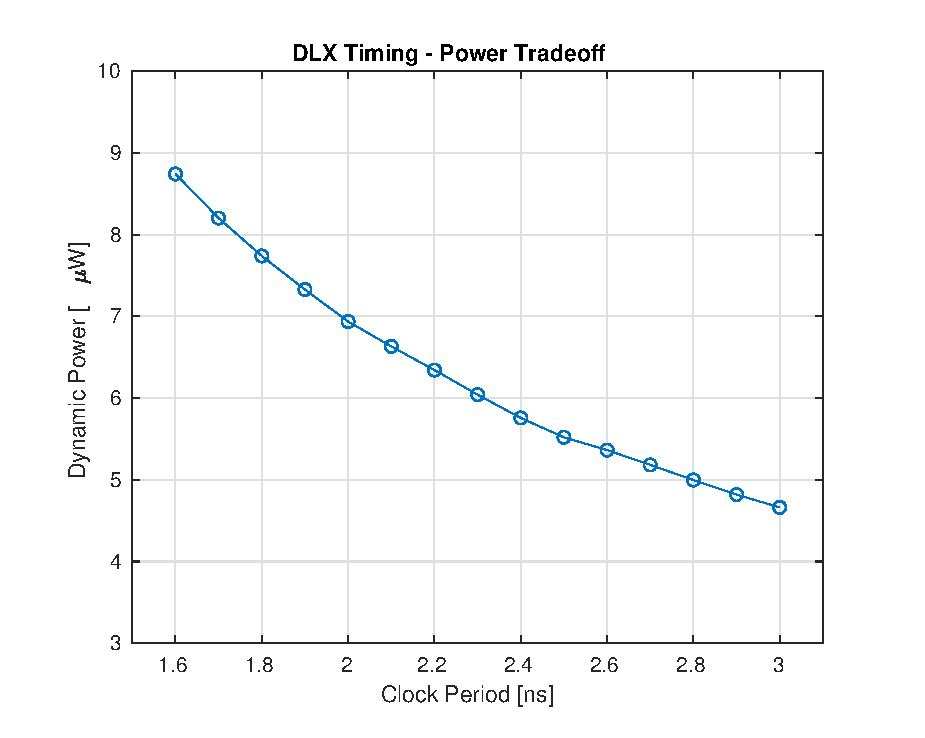
\includegraphics[width=0.8\textwidth, center]{images/PPA.eps}
	\caption{DLX - Timing/Power Tradeoff Curve - Clock Gating Enabled}
	\label{PPA}
\end{figure}


\section{Layout}\label{Layout}
\begin{figure}[!ht]
	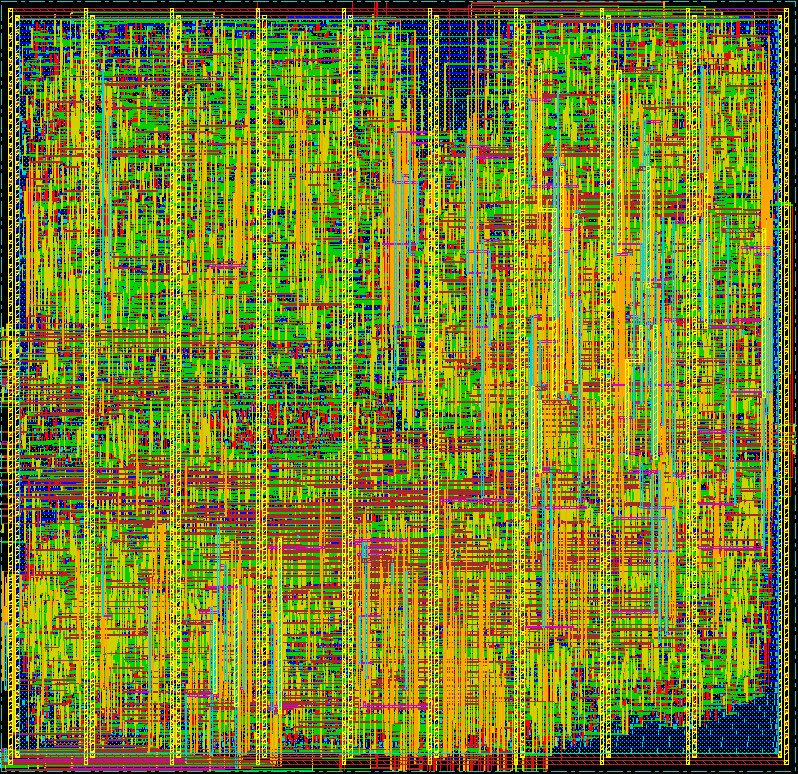
\includegraphics[width=0.8\textwidth, center]{images/dlx-floorplan.jpg}
	\caption{DLX - Post Place\&Route Schematic from Encounter}
	\label{FLORPLANR}
\end{figure}
Finally as our last step, Physical design of the entire processor has been done. We followed the same procedure as the one described in the laboratory instruction, because we don't know the Encounter tool very well.

We decided to do the Floorplanning only for the non-clock-gated design with clock period of 1.6 ns.

Due to the large size of the design, some processes took a lot of time, for example Clock Tree Synthesis and Cell Placement.

At the end we printed all the reports, luckily our design show no geometry or connectivity violations.
Only some hold timing violations appear to be present.


Among all the reports, we extracted some values regarding gate count and area:
\begin{table}
\begin{center}
	\begin{tabular}{ | c | c | c | c |}
		\hline
		\rowcolor{LimeGreen}   Block & Gate Count & Area($\mu m^2$)& \%\\ \hline
		Total & 26524 & 21166.7 & 100\% \\ \hline
		Register File & 10444 & 8334.3 & 39\% \\ \hline
		BTB & 6401 &  5108.0 & 24\% \\ \hline
		ALU & 4088 & 3262.2 & 15\% \\ \hline
	\end{tabular}
	\caption{DLX - Post Place\&Route Gate Count and Area}
	\label{AREA}
\end{center}
\end{table}
It's interesting to see that more than 60\% of the overall area is occupied by BTB and Register File.



\section{Conclusions}\label{Conclusions}
This project required a incredible amount of work and taught us that microelectronic design is not so simple.

As a future work, this design could be extended by including the missing instructions and adding the Floating Point part of the microprocessor. 
Also it would be interesting to see some numbers regarding the branch predictor, in particular a tradeoff curve between size and misprediction rate with real life benchmarks.


\printbibliography

\begin{landscape}
	\begin{figure}[!ht]
		\includegraphics[height=1\textheight,center]{images/SCHEME_DLX_FW.eps}
		\caption{DLX - Full Datapath Scheme}
		\label{PPA}
	\end{figure}
	\end{landscape}

\end{document}